\documentclass[english]{beamer}
\usepackage[T1]{fontenc}
\usepackage{graphicx}
\usepackage{adjustbox}
\usepackage{verbatim}
\usepackage{booktabs}
\makeatletter
\newcommand\makebeamertitle{\frame{\maketitle}}%
\makeatother
\begin{document}
\begin{frame}{afqtMeanByQual.pdf}
\begin{center}
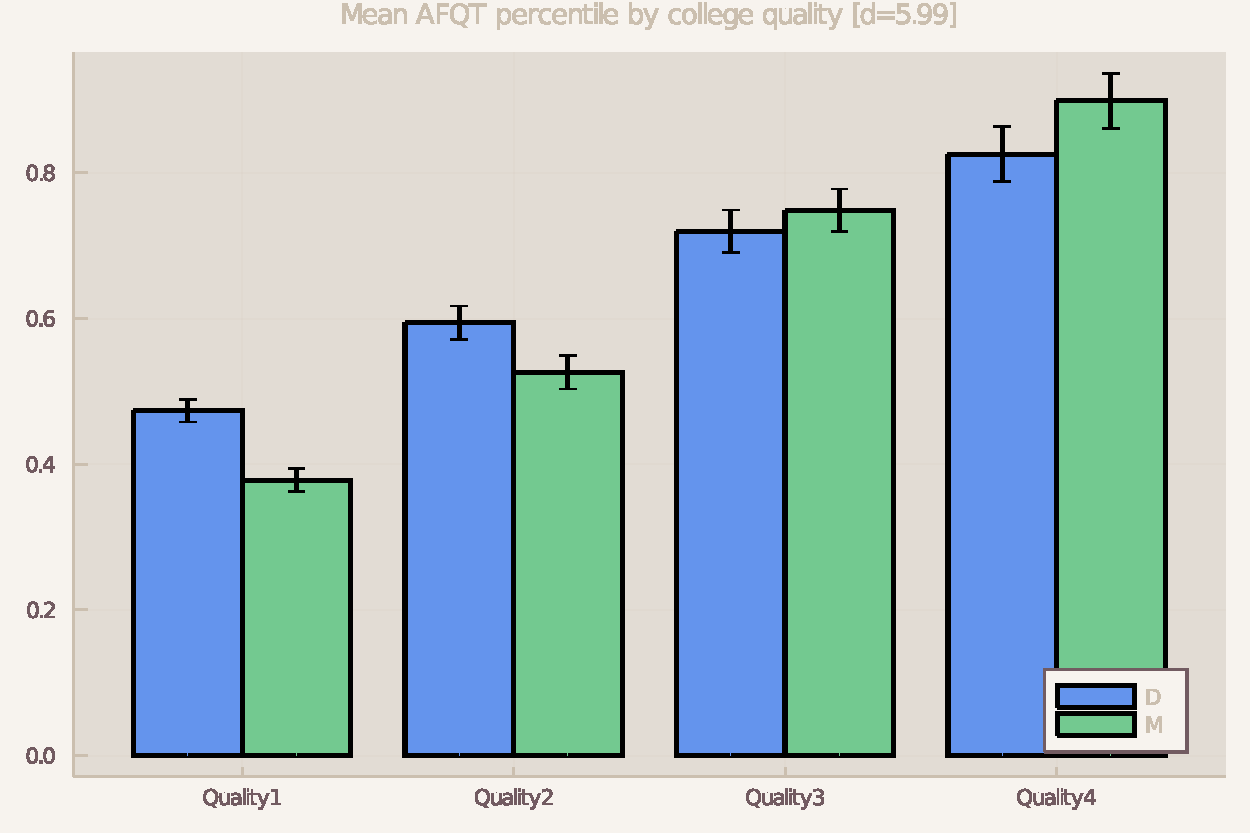
\includegraphics[width=0.95\textwidth]{/Users/lutz/Documents/julia/LatexLH/test/test_files/afqtMeanByQual.pdf}
\end{center}
\end{frame}
\begin{frame}{fracGradByQual.pdf}
\begin{center}
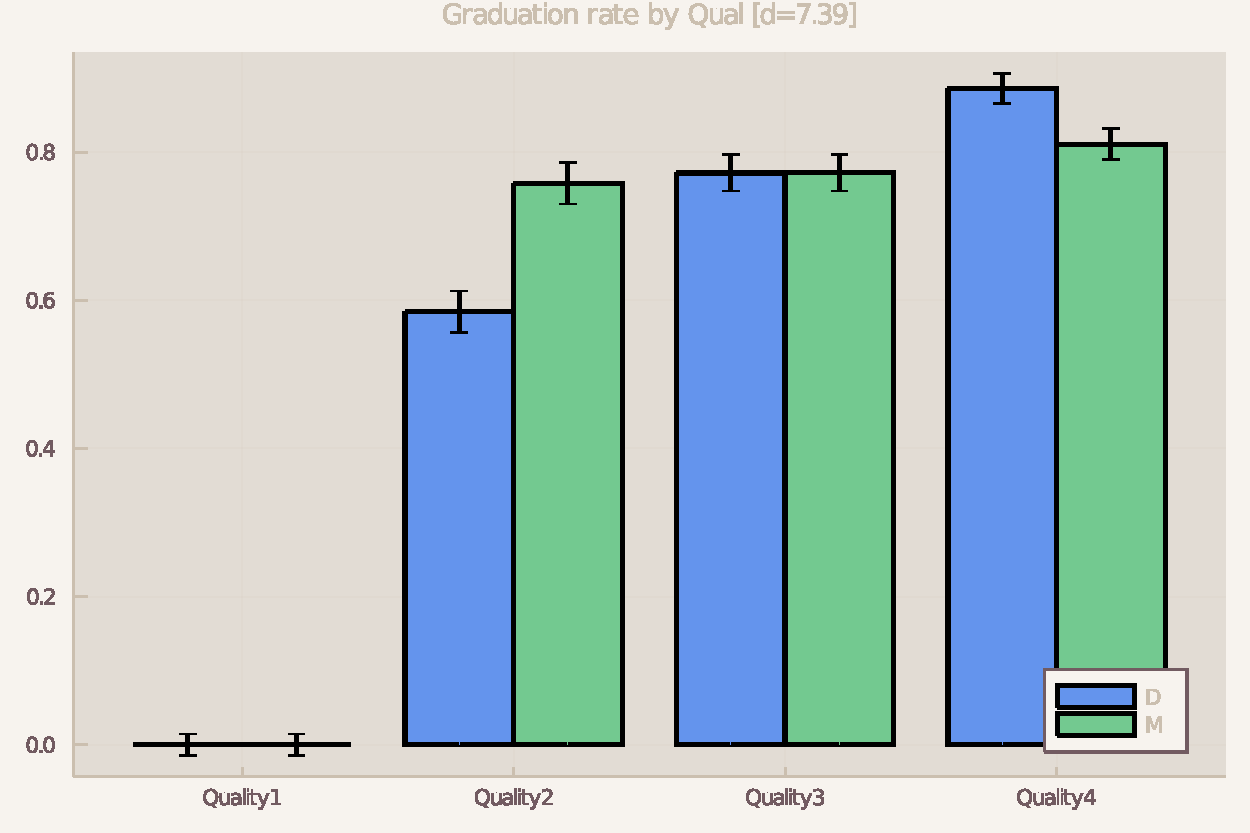
\includegraphics[width=0.95\textwidth]{/Users/lutz/Documents/julia/LatexLH/test/test_files/fracGradByQual.pdf}
\end{center}
\end{frame}
\begin{frame}{parameter\_table\_test.tex}
\begin{table}[h]
\centering
\begin{adjustbox}{width=1\textwidth}
\begin{tabular}{lll} 
\toprule 
Parameter & Description & Value \\ 
\midrule 
p1 & param 1 & 1.23 \\ 
p2 & param 2 & 2.34 \\ 
\bottomrule 
\end{tabular} 

\end{adjustbox}
\end{table}
\end{frame}
\end{document}
